% Preamble
% =============================================================================

% Class of the document.
\documentclass[12pt,a4paper]{article}
% article : short article.
% report  : mid-length report.
% book    : book or thesis redaction.

% Paragraph skip length (default to 0).
\setlength{\parskip}{1ex}

% Packages
% =============================================================================

% Encoding
% -----------------------------------------------------------------------------

% Babel.
\usepackage[french]{babel}
% FontEnc.
\usepackage[T1]{fontenc}
% InputEnc.
\usepackage[utf8]{inputenc}

% Define \escapeus command to escape underscores.
\makeatletter
\DeclareRobustCommand*{\escapeus}[1]{
    \begingroup\@activeus\scantokens{#1\endinput}\endgroup}
\begingroup\lccode`\~=`\_\relax
    \lowercase{\endgroup\def\@activeus{\catcode`\_=\active \let~\_}}
\makeatother

% Text
% -----------------------------------------------------------------------------

% Acronym.
\usepackage{acronym}
% CsQuote.
\usepackage[style=french,french=guillemets]{csquotes}
% Enumerate.
\usepackage{enumerate}
% HyperRef.
\usepackage[hyperfootnotes=false,hidelinks]{hyperref}
% URL.
\usepackage{url}

% Algorithms
% -----------------------------------------------------------------------------

% Algorithm2E.
\usepackage[french,onelanguage,linesnumbered,ruled,vlined,commentsnumbered]{algorithm2e}

% Source code
% -----------------------------------------------------------------------------

% Listings.
\usepackage{listings}
% Minted.
\usepackage{minted}
% Caption.
\usepackage{caption}
\newenvironment{code}{\captionsetup{type=listing}}{}

% Files
% -----------------------------------------------------------------------------

% FancyVRB.
\usepackage{fancyvrb}
% Redefine \VerbatimInput.
\RecustomVerbatimCommand{\VerbatimInput}{VerbatimInput}
{
    fontsize=\footnotesize,
    frame=lines,         % Top and bottom rule only.
    framesep=1.5em,      % Separation between frame and text.
    rulecolor=\color{red!50!green!50!blue!50!},
    labelposition=topline,
    commandchars=\|\(\), % Escape character and argument delimiters for commands within the verbatim.
    commentchar=*        % Comment character.
}

% Figures
% -----------------------------------------------------------------------------

% GraphicX.
\usepackage{graphicx}
% SVG.
\usepackage{svg}
% WrapFig.
\usepackage{wrapfig}

% Charts
% -----------------------------------------------------------------------------

% PGFPLots
\usepackage{pgfplots}
\pgfplotsset{compat=1.16}
\usepgfplotslibrary{units}

% Mathematics
% -----------------------------------------------------------------------------

% AmsFonts.
\usepackage{amsfonts}
% AmsMath.
\usepackage{amsmath}
% AmsText.
\usepackage{amstext}
% AmsThm.
\usepackage{amsthm}
\newtheorem{prr}{Propriété}
\newtheorem{pro}{Proposition}
\newtheorem{thm}{Théorème}
\newtheorem{lem}{Lemme}
% NumPrint.
\usepackage{numprint}

% Physics
% -----------------------------------------------------------------------------

% Physics.
\usepackage{physics}

% Presentation
% -----------------------------------------------------------------------------

% XColor.
\usepackage{xcolor}

% References
% -----------------------------------------------------------------------------

% CleveRef.
\usepackage{cleveref}

% Structure.
% -----------------------------------------------------------------------------

% Geometry.
\usepackage{geometry}
% PDFLScape.
\usepackage{pdflscape}
% MultiCol.
\usepackage{multicol}
% TitleSec.
\usepackage{titlesec}
\newcommand{\sectionbreak}{\clearpage} % Use a page break before new sections.
% VMargin.
\usepackage{vmargin}
% FootMisc.
\usepackage[bottom]{footmisc}

% Symbols
% -----------------------------------------------------------------------------

% SIUnitX.
\usepackage{siunitx}

% Table
% -----------------------------------------------------------------------------

% Array.
\usepackage{array}
% BookTabs.
\usepackage{booktabs}
% CSVSimple.
\usepackage{csvsimple}

% Document
% =============================================================================

\begin{document}

\title{Projet Réseau}
\author{Pierre AYOUB -- Océane FLAMANT}

\maketitle

\begin{figure}[b]
    \centering
    
\includegraphics[scale=0.3]{figures/isty.jpg}
\end{figure}


\tableofcontents

\section{Introduction}
\label{sec.intro}
Afin d'éviter les coupures de l'Internet des Objets il est nécessaire de 
trouver des solutions automatisées. Cela permettrait aux équipements 
d'être autonome dans un environnement dynamique.
Dans ce projet, nous allons appliquer ce concept au contexte des réseaux 
émergents LoRaWAN. Pour cela on va utiliser un algorithme d'apprentissage par
renforcement de type bandit manchot. De plus afin d'accélérer la convergence 
de l'algorithme nous n'utiliserons que deux canaux et trois facteurs 
d'étalement.



\section{Explication du code}
\label{sec.expl}

Pour réaliser ce projet, implémenter l'algorithme, nous avons d'abord dû 
réfléchir aux structures de données et aux fonctions dont nous aurions 
besoin ainsi qu'à l'initialisation de certaines données.

\subsection{Structures données}
\label{sub.exp.struct}
La formule utilisée et certaines contraintes nécessite de conserver plusieurs données :
\begin{description}
    \item[La moyenne de la machine] Il faut conserver tous les 
    choix de chaque machine à chaque tour. Pour ce faire nous avons décidé
    de créer une structure "tour" qui est composée du canal et du facteur 
    d'étalement choisit ainsi que de la valeur (s'il y a eu collision 0 et 
	un valeur inversement proportinel au SF sinon).
    La moyenne est calculée pour toutes les combinaisons mais une seule est 
    choisie à chaque tour donc il ne faudra recalculer qu'une seule valeur
    c'est pour cela que nous avons décidé que chaque machine posséderais 
    un tableau qui contiendra la moyenne de chaque combinaison.
    \item[Le nombre d'utilisation de la machine] Il faut savoir pour chaque 
    combinaison combien de fois elle a été utilisé. Pour cela nous avons 
    pris la décision encore une fois de stocker ces valeurs dans un tableau.
    \item[La position des équipements] En effet, en fonction de sa position 
    un équipement n'a pas forcement accès au même facteur d'étalement c'est 
    pour cela que nous conservons cette donnée dans un tableau.
\end{description}
Pour finir nous avons décidé de réunir toutes ces données dans une seule 
structure"gain" afin de faciliter la compréhension du code et pour facilité 
la manipulation des données.

\subsection{Fonctions}
\label{sub.exp.fct}
Ensuite nous avons réfléchi aux fonctions que nous devions implémenter et 
nous en avons trouvé trois : 
\begin{itemize}
	\item Une pour initialiser à une valeur précise certains tableaux.
	\item Une autre pour calculer la moyenne.
	\item Une pour calculer quelle combinaison serait la
	plus efficace pour la machine donnée. Cette fonction choisit la combinaison
	dont l'envoie du paquet à le plus de chance de réussir. Si deux ou 
	plus on la même chance alors on en prend une au hasard.
	\item Et enfin une dernière qui choisit aléatoirement une combinaison.
	Cette fonction nous permettra de faire une comparaison avec la fonction 
	précedente et ainsi voir si nous avons pu améliorer le nombre de paquet
	envoyé.
\end{itemize}
\subsection{Initialisation}
\label{sub.exp.struct}
Passons maintenant à l'initialisation des données. Nous avons décidé 
d'initialiser la moyenne de chaque combinaison utilisable à 1 afin d'obliger le 
programme à choisir au moins une fois chaque combinaison disponible. 
Les combinaisons qui ne doivent pas être utilisées sont initialisées à moins 
un. Nous ne pouvions pas l'initialiser à 0 sinon le programme ne prendrait 
toujours la même combinaison. On initialise aussi le nombre de fois que 
la combinaison a été utilisé à un car sinon avec la formule cela peut créer 
une division par 0. De plus il faut, pour le compte du nombre de tour, faire 
attention a bien commencé a un sinon, à cause de la formule encore une fois, 
on va avoir log(0). Pour positionner les équipements dans les trois cercle nous 
avons utilisé le hasard. 

\section{Résultat}
\label{sec.res}
Une fois le programme implémenté il a fallu le tester et voir si les résultats
nous semblaient corrects. Pour cela nous avons décidé de ne faire varier 
que le nombre d'équipements de 5 à 10 et de garder constant le nombre de tours 
sachant que le nombre de combinaisons possible est 6.
Pour chaque nombre d'équipements nous avons exécuté le programme 20 fois afin 
d'avoir une moyenne et non pas une valeur unique pour que notre résultat soit
le plus fiable possible.
\newline
Afin de pouvoir mieux observer la différence entre les deux méthodes nous 
avons décidé d'utiliser un graphique.
\newline Dans les deux cas, plus le nombre 
d'équipements augmente plus le nombre de paquets envoyés diminue. Cela nous 
semble cohérent puisque une fois que les six combinaisons ont été choisit 
plus aucun paquet ne peut passer cela pose moins de problèmes tant que le nombre
d'équipements souhaitant envoyer un paquet est inférieur au nombre de 
combinaison possible car les équipements ont toujours la possibilité de 
choisir une combinaison non utilisée alors que quand le nombre d'équipement 
est plus élevé que le nombre de combinaisons, les derniers équipements n'ont 
presque aucune chance d'avoir encore une combinaison de disponible.
\newline On remarque cependant qu'en utilisant la méthode bandit manchot 
quand le nombre de combinaisons est inférieur au nombre d'équipements alors 
cette méthode est bien plus efficace et entraine bien moins de collision. Le 
programme sait quelle combinaison choisir pour réduire le nombre de colisions.


\begin{figure}[h]
    \centering
    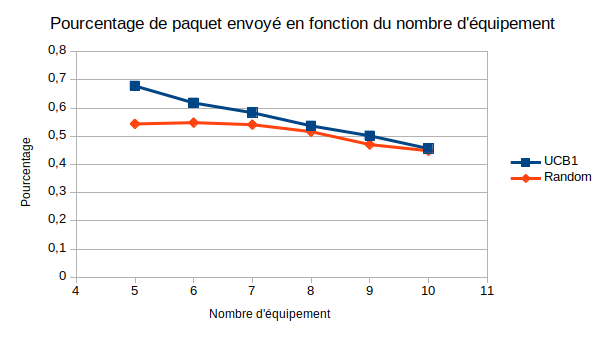
\includegraphics[scale=1]{figures/graphe.png}
\end{figure}



\end{document}
